\documentclass[a4paper, 10pt]{article}
% Packages
\usepackage[utf8]{inputenc}  % For Unicode support
\usepackage{amsmath}         % For math symbols
\usepackage{graphicx}        % For including images
\usepackage{hyperref}        % For hyperlinks
\usepackage{graphicx}        % For image rendering
\usepackage{listings}        % For code blocks
\usepackage{sectsty}         % For section font formatting
\usepackage[a4paper, total={7in,9.5in}]{geometry} % For Margins
\usepackage{xcolor}
\usepackage{hyperref}
\usepackage{mathptmx}

% Package Initialization
\graphicspath{{~/courses/algorithms/notes/images/}}

% Formatting
\sectionfont{\fontsize{16}{14}\selectfont}
\hypersetup{
    colorlinks=true,
    linkcolor=blue,
    filecolor=magenta,
    urlcolor=cyan,
}
% Define the style for C++ code
\lstdefinestyle{cpp}{
    language=C++,
    basicstyle=\ttfamily\small,
    keywordstyle=\color{blue},
    stringstyle=\color{red},
    commentstyle=\color{gray},
    morecomment=[l][\color{magenta}]{\#},
    % numbers=left,
    numberstyle=\tiny\color{gray},
    stepnumber=1,
    numbersep=8pt,
    showstringspaces=false,
    breaklines=true,
    % frame=single,
    rulecolor=\color{black},
    backgroundcolor=\color{white},
    tabsize=2,
    captionpos=b
}

% Title, author, date
\title{A Tour of C++}
\author{ksolomon}
\date{\today}

\begin{document}

\maketitle

\begin{abstract}
	Notes on Algorithms Course Pt 1
\end{abstract}


%%%%%%%%%%%%%%%%%%%%%%%%%%%%%%%%%%%%%%%%%%%%%%%%%%%%%%%%%%%%
% Chapter 1 - Introduction
%%%%%%%%%%%%%%%%%%%%%%%%%%%%%%%%%%%%%%%%%%%%%%%%%%%%%%%%%%%%

\section{Introduction}
Highly recommend to code up every single algorithm presented in the course in favorite programming language to fully grasp the concepts.
\begin{quote}
	\centering
	\textit{"Perhaps the most important principle for the good algorithm designer is to refuse to be content" - Aho, Hopcroft, and Ullman , The Design and Analysis of Computer Algorithms, 1974}
\end{quote}
\subsection{Multiplication}
\paragraph{Integer Multiplication}
Grade school algorithm is $O(n^2)$.
\paragraph{Karatsuba Multiplication}
\newtheorem{theorem}{Theorem}
\begin{theorem}
	let \(x = 5678, y = 1234\)

	let \(a = x / 100, b = x mod 100\)

	let \(c = y / 100, d = y mod 100\)
	\begin{enumerate}
		\item a*c = 672
		\item b*d = 2652
		\item (a+b)(c+D) = 134*46 = 6164
		\item (3) - (2) - (1) = 2840
		\item (1)*10000 + (2) + (4)*100 = 6720000 + 2652 + 284000 = 7006652
	\end{enumerate}
\end{theorem}
\begin{figure}[ht]
	\centering
	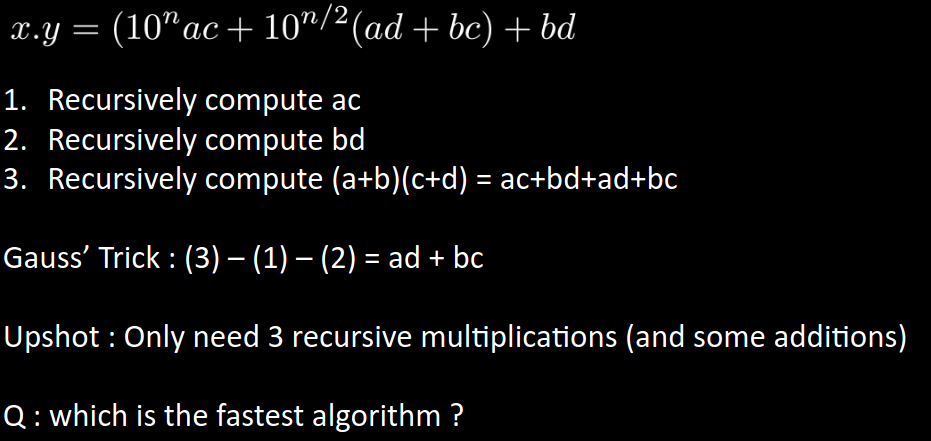
\includegraphics[width=0.7\textwidth]{intro.karatsuba.png}
	\caption{Recursive Karatsuba Multiplication}
\end{figure}

\end{document}
